\documentclass[parskip=full, DIV=14]{scrartcl}

\usepackage[T1]{fontenc}
\usepackage{selinput}% Eingabecodierung automatisch ermitteln siehe <http://ctan.org/pkg/selinput>
\SelectInputMappings{
	adieresis={ä},
	germandbls={ß},
} 
\usepackage{ngerman}

\usepackage{amsmath}

\usepackage{graphicx}
\graphicspath{{Bilder/}}

\usepackage{listings}
\usepackage[dvipsnames]{xcolor}

\lstset{language={Java},
        numbers=left,
        stepnumber=1,
        numbersep=5pt,
        numberstyle=\tiny,
        breaklines=true,
        breakautoindent=true,
        postbreak=\space,
        tabsize=2,
        basicstyle=\ttfamily\footnotesize,
        showspaces=false,
        showstringspaces=false,
        extendedchars=true,
        commentstyle=\color{Gray}, % comment color
    	keywordstyle=\color{Bittersweet}, % keyword color
    	stringstyle=\color{red}, % string color
        % Sorgt dafür, dass das Paket listings auch mit den Sonderzeichen in UTF-8 zurecht kommt.
				literate=
					{Ö}{{\"O}}1
					{Ä}{{\"A}}1
					{Ü}{{\"U}}1
					{ß}{{\ss}}2
					{ü}{{\"u}}1
					{ä}{{\"a}}1
					{ö}{{\"o}}1
        }

\usepackage[hidelinks]{hyperref}

\newcommand{\shellcmd}[1]{\texttt{\$ #1}\\}

\begin{document}
	\titlehead{35. Bundeswettbewerb Informatik \hfill Team 00001, Teilnahme 6745}
	\title{Rhinozelfant}
	\subtitle{Aufgabe 2}
	\author{Laurenz Friedrich Grote \& Jon Amos Fehling}
	\date{}
	\maketitle
	\tableofcontents
	
	\vspace {3em}

	Meine Umsetzung für "`Rhinozelfant"' erfolgte unter Arch Linux mit Java 1.8. Der Programmcode liegt sowohl als ausführbare JAR-Datei als auch als Quellcode vor. Der Quellcode unterstützt nur PNG-Dateien.

	Bitte beachten Sie, dass im Normalfall die GUI sich öffnet, Sie jedoch auch auf der Kommandozeile ein Einzelbield analysieren können:

	\shellcmd{java -jar Rhinozelfant.jar -{}-cmd QUELLE ZIEL}

	\clearpage
	% ----------------------------------------------------------------------------
	\section{Lösungsidee}
		Die Aufgabenstellung habe ich in foglende Teilaufgaben eingeteilt:
\begin{enumerate}
	\item Finden der mögichen Hautschuppen
	\item Filtern, welche der Hautschuppen tatsächlich zu einem Rhinozelfanten gehören
	\item Einfärben des gesamten Rhinozelfanten
\end{enumerate}

Eine Hautschuppe haben wir als Pixel definiert, das mehr als 2 gleichfarbige Nachbarfelder hat. Nachbarfelder sind alle direkt und diagonal anliegenden Pixel.

Diese Hautschuppenmenge enthält allerdings noch einige vermeintliche Hautschuppen, die zu keinem Rhinozoelefanten gehören. Beispielsweise werden oft Pixel im Himmel als Hautschuppe erkannt, da nur wenige Blautöne vorliegen. Diese False Positives müssen für ein besseres Ausgabebild herausgefiltert werden.

Dazu haben wir zuerst das Problem vereinfacht: Anstatt dies direkt auf dem bunten Bild durchzuführen, wird ein Schwarz-Weiß-Bild erstellt. In diesem Bild sind schwarze Pixel mögliche Hautschuppen, weiße Felder sind auf keinen Fall Hautschuppen. Dieses Zwischenbild wird Ihnen in der GUI angezeigt.

Auf dieses werden folgende Filter angewandt, um zu bestimmen welche möglichen Hautschuppen tatsächlich Teil eines Rhinozelfanten sind.

\begin{description}
	\item[Linienfilter] Zuerst wird nach ausreichend großen durchgehenden Linien gesucht: Einzelne Hautschuppen können schließlich keine Rhinozelfanten sein. Wir haben festgelegt, dass ein Rhinozelfant an seiner dicksten Stelle 4\% der Gesamtbreite des Bildes haben muss. Dies überschreiten alle Rhinozelfanten in den Beispielen deutlich. Kleinere Werte würden die Laufzeit erheblich verlängern, da mehr mögliche Rhinozelfanten an die nachfolgenden Filter weitergegeben werden würden. Größere Werte würden dementsprechend den Programmablauf beschleunigen, es könnten jedoch Rhinozelfanten übersehen werden. Alle Linien, die dieses Kriterium erfüllen, werden an den nächsten Filter weitergegeben.
	\item[Rechteckfilter] In den Bauch eines Rhinzelfanten lässt sich ein Rechteck zeichnen. In diesem Schritt wird überprüft, ob sich mit der soeben gefundenen Linie als obere Kante ein Rechteck höher als 1,25\% der Gesamthöhe des Bildes zeichnen lässt. Alle Rechtecke, die dieses Kriterium erfüllen, werden an den nächsten Filter weitergegeben.
	\item[Anatomiefilter] Zuletzt wird überprüft, ob sich das Umfeld des Rechteckes mit der Anatomie eines Rhinozelfanten deckt. Dazu wird überprüft, ob sich an das Rechteck Beine anzeichnen lassen. Auf den Rüssel wird nicht eingegangen, da seine Position stark variiert und die drei vorher genannten Filter keine False Positives gefunden haben.
\end{description}

Wenn von einer Stelle ausgehend all diese Kriterien zutreffen, sind alle zusammenhängenden Hautschuppen ein Rhinozelfant. Zwei Hautschuppen hängen zusammen, wenn sie benachbart sind.

\clearpage
Beispiel: \vspace{3em}
\begin{figure}[!ht]
	\centering
	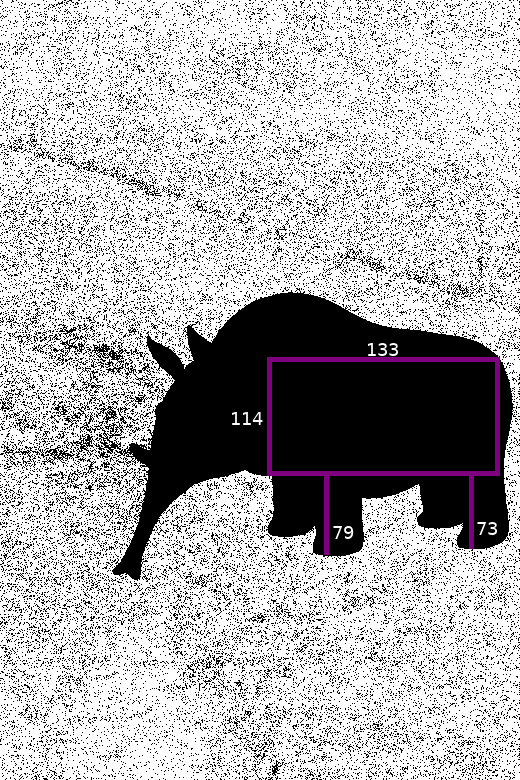
\includegraphics[width=0.7\textwidth]{SkizzeIdee4}
	\caption {Bsp. 4. mit eingezeichneten Skelett}
	Um den Filtereffekt zu verdeutlichen, wurde jedes Pixel mit mehr als einem gleichfarbigen Nachbar markiert.
\end{figure}
	\clearpage
	\section{Umsetzung}
		Die 3 Aufgaben aus der Lösungsidee haben wir in zwei Java-Klassen aufgeteilt. Alle Funktionen, die mit dem eigentlichen farbigem Bild interagieren finden sich in der Klasse Bild (Schritte 1 und 3), die, die mit der Abstraktion arbeiten, liegen in der Klasse RhinozelfantenSucher (Schritt 2).

	\subsection {Suche nach möglichen Hautschuppen}

	Die Suche nach möglichen Hautschuppen findet mit Brute-Force statt. Das heißt für jedes Pixel wird die Farbe mit den 9 umliegenden Pixeln verglichen. Sind mehr als zwei der umliegenden Felder gleichfarbig, handelt es sich um eine mögliche Hautschuppe. Das in der Lösungsidee beschriebene S/W-Bild für die nächsten Schritte haben wir als zweidimensionales Bool-Array realisiert. True entspricht schwarz (mögliche Hautschuppe), False weiß (keine Hautschuppe). 

	In der GUI wird dieses S/W-Bild zu Debugzwecken angezeigt. Da die Filter das Array manipulieren werden, wird, sofern die entsprechende Debug-Flag gesetzt wurde, an dieser Stelle eine Deep Copy des Arrays gezogen.

	\subsection {Filterprozess}
	Nachdem nun das S/W-Bild an die Klasse RhinozelfantSucher übergeben wurde, werden die Hautschuppen, die tatsächlich Teil eines Rhinozelfanten sind, herausgefiltert. Jeder der drei Filter ist als eine eigene Methode innerhalb von RhinozelfantenSucher implementiert.

		\subsubsection{unterbrechungsfreieStricheFilter()}

		Nach der Lösungsidee ausreichend lange Linien findet das Programm, indem es in jeder Zeile die Länge aufeinanderfolgende True-Bereiche zählt. Überschreitet die Länge eines Bereiches die Mindestlänge, wird die 1. und 2. x-Position \texttt{(startX, endeX)} sowie die Zeile \texttt{(endeY)} an den nächsten Filter weitergeben.

		\subsubsection{rechteckFilter (int startX, int endeX, int startY)}

		In dieser wird Funktion überprüft, ob eine Zeile tiefer ebenfalls zwischen \texttt{startX} und \texttt{endeX} der davor gefundenen Linie sich eine Linie aus möglichen Hautschuppen befindet. Wenn dies der Fall ist, könnte zwischen \texttt{startY} (der oberen Kante) und der darunterliegenden Zeile ein Rechteck nur aus möglichen Hautschuppen gezeichnet werden. 

		Die untere Kante des Rechteckes wird solange nach unten verschoben, bis sich entweder eine Zeile findet, in der sich zwischen \texttt{startX} und \texttt{endeX} nicht ausschließlich mögliche Hautschuppen vorliegen oder die letzte Zeile erreicht ist.
		
		Überschreitet die Höhe des Rechtecks, also \(startY - endeY\), die in der Lösungsidee genannte Mindesthöhe, bedeutet dies, dass unter den im 1. Schritt gefundenen Strich ein "`Bauch"' gezeichnet werden kann. Dann werden die Koordinaten der unteren Kante des Recheckes an den letzten Filter weitergeben.

		\subsubsection{anatomieFilter (int startX, int endeX, int y)}
		Dies ist der Hauptfilter, der leider auch recht laufzeitintensiv ist. Deshalb wurden in den vorherigen Filtern bereits die meisten Stellen ausgeschlossen. 

		Hier wird überprüft, ob an das soeben gefundene Rechteck Beine anliegen. Hierzu wird zunächst im ersten und letzten Drittel der unteren Kante des Rechteckes der längste nach unten gehende Strich (Bein) bestimmt.

		Dies erfolgt indem, ähnlich wie beim vorherigen Filter, von jeder möglichen x-Koordinate im ersten und letzten Drittel überprüft wird, um wieviele Zeilen man einen Zeiger nach unten verschieben kann, ohne dass ein Pixel keine mögliche Hautschuppe (False) ist.
		
		Überschreiten beide Striche das Minimum von 4px, wird ferner noch überprüft, ob zwischen den beiden Beinen ein Zwischenraum liegt, da bei einem Lebewesen sich zwischen den Hautschuppen der Beine Luft befindet. Dies wird durchgeführt, indem zwischen dem kürzeren Bein und dem gegenüberliegenden Bein ein Zeiger solange verschoben wird, bis auf eine Luftzelle gestoßen wird.

		Stimmen all diese Bedingungen zu, ist um das gefundene Rechteck die Anatomie eines Rhinozelfanten gegeben. Im nächsten Schritt wird der gesamte Elefant weiß markiert.

	\subsection {Gesamtstruktur suchen}
	Die zuerste geplante Lösung mithilfe von Rekursion funktionierte leider nicht, da es bei den Testcases (6. Mio. Pixel) zu einem Pufferüberlauf kam.

	Daher haben wir uns für eine iterative Lösung entschieden:

	Jedes Feld, mit der vom anatomieFilter übergebenen Urpsrungskoordiante angefangen, wird zunächst einem Stapel mit allen Koordinaten des Rhinozelfanten, die noch nicht bearbeitet wurden, hinzugefügt. Außerdem wird die Stelle im 2D-Bild auf False gesetzt, damit es bei der weiteren Suche nicht zu Endlosschleifen kommt.

	Darauf wird für jede Koordinate im Stapel folgendes durchgeführt:

	\begin{enumerate}
		\item Diese Koordiante wird auf eine Liste mit den einzufärbenden Bildern gesetzt
		\item Alle direkt anliegenden True-Feldern sind ebenfalls Teil der Rhinozoelefantenstruktur und werden deshalb, wie das Ursprungsfeld, nun als False markiert und dem Stapel hinzugefügt.
	\end{enumerate}

	So werden alle aneinander angrenzenden gleichfarbigen Felder des Rhinozelfanten markiert. Die Liste ist ein Klassenobjekt das nach Ablauf aller Filter von der Bildklasse aberufen wird. Diese kann dann alle gefunden Elefanten im RGB-Bild einfärben.

	\subsection {Markieren der Flächen}

	Da von der letzten Stelle alle zu Rhinozoelefanten gehörenden Punkte als Arraylist ausgegeben wurden, können diese nun einfach Punkt für Punkt im BufferedImage weiß markiert werden.
	\section{Überlegungen zur Laufzeit}
		Die Laufzeit des Programmes wächst ungefähr linear zu der Gesamtpixelzahl des Bildes, da der Großteil der Laufzeit für die Suche nach möglichen Hautschuppen und das Auszählen der Linienlängen genutzt wird.

Die Beschaffenheit (Anzahl möglicher Hautschuppen) spielt im Average-Case eine eher geringe Rolle, da die meisten Pixel bei der Hautschuppensuche und der Linienananlyse mit jeweils konstanter Laufzeit ausgeschlossen werden können.

Im Best-Case, also einem Bild aus zufälligem Rauschen, in dem keine Filter zum Einsatz kommen, benötigt das Programm für 6 Mio. Pixel (2000x3000) 2.3s. 
Wenn nun in einem Average-Case (Bsp. 4) einige Filterausführungen zum Finden eines im Bild vorhandenen Rhinozelfanten benötigt werden, steigt die Laufzeit marginal auf 2.6s an. 
Im Worst-Case, nämlich einem komplett einfarbigen Bild, in dem alle Pixel mögliche Hautschuppen sind, werden zahlreiche komplette Filterdurchläufe benötigt, die Laufzeit beträgt dann 30s.
	\clearpage
	\section{Beispiele}
		Beispielausgaben aller auf bwinf.de zur Verfügung gestellten Beispiele finden Sie im .zip.

Hier finden Sie die Ausgaben, auf denen ein Rhinozelfant gefunden wurde. Die Bilder auf denen kein Rhinozelfant gefunden wurde, entsprechen zu 100\% den Eingabebildern.

\subsection{Beispiel 1}
	\centering
	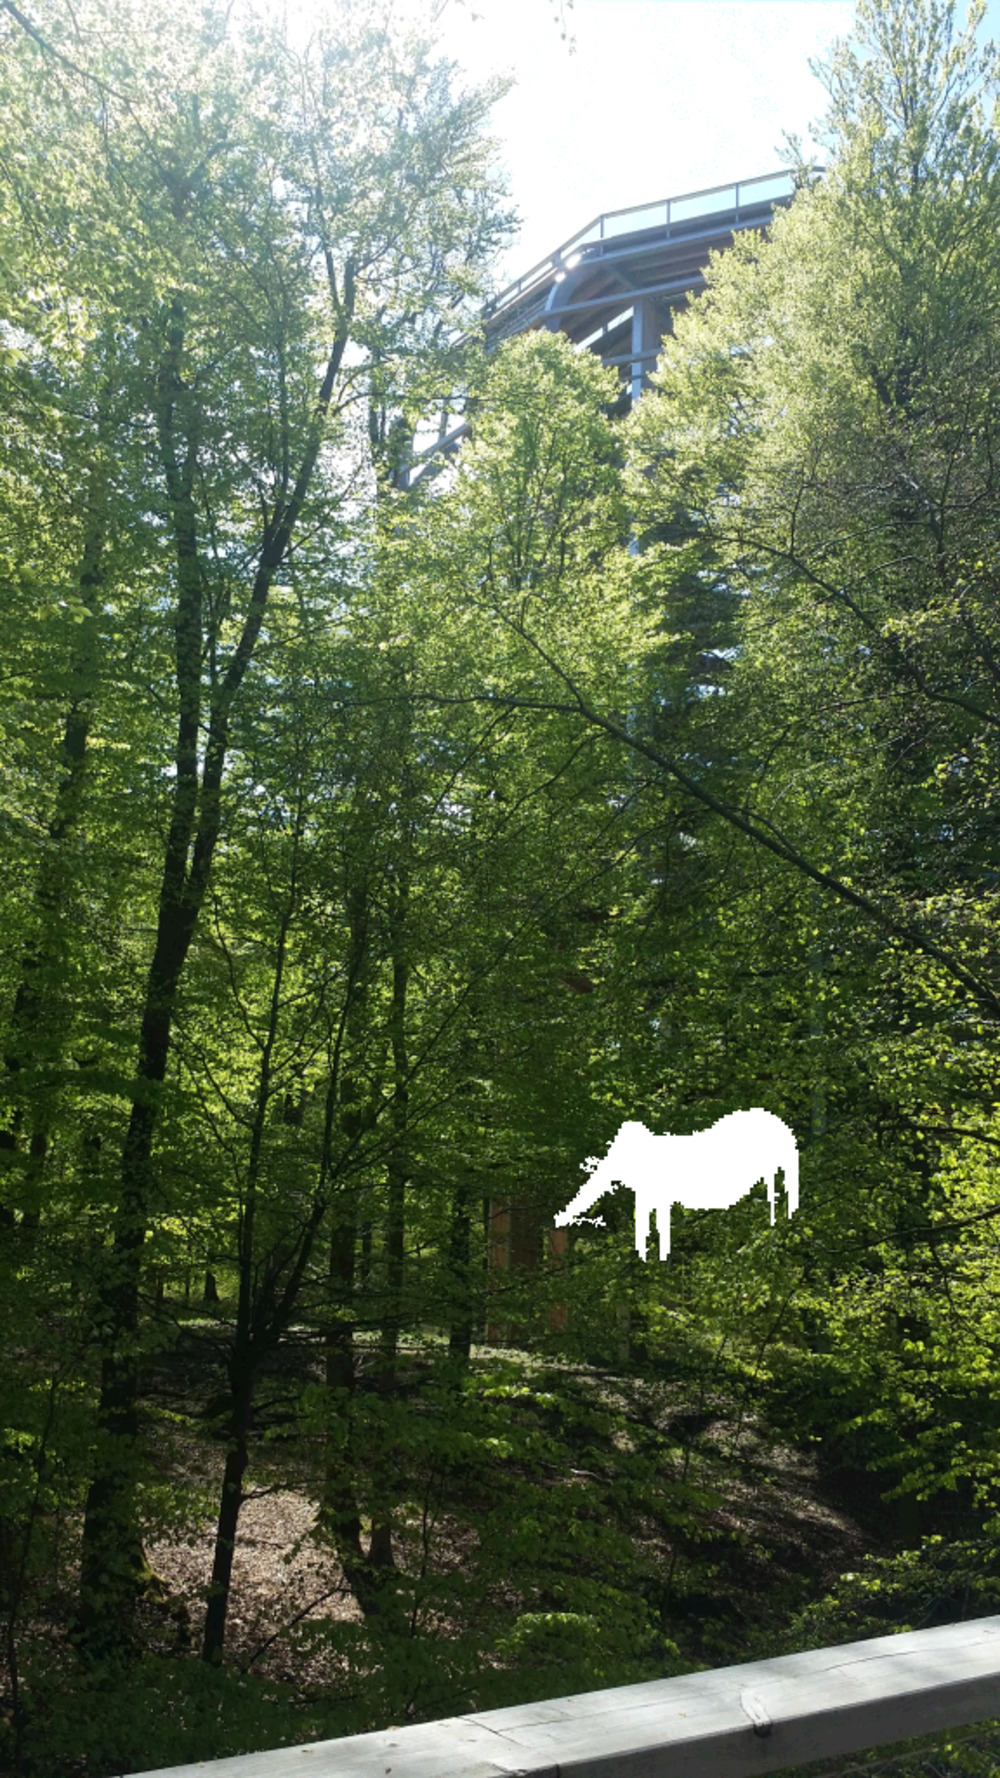
\includegraphics[width=0.45\textwidth]{bsp-0}
\subsection{Beispiel 2}
	\centering
	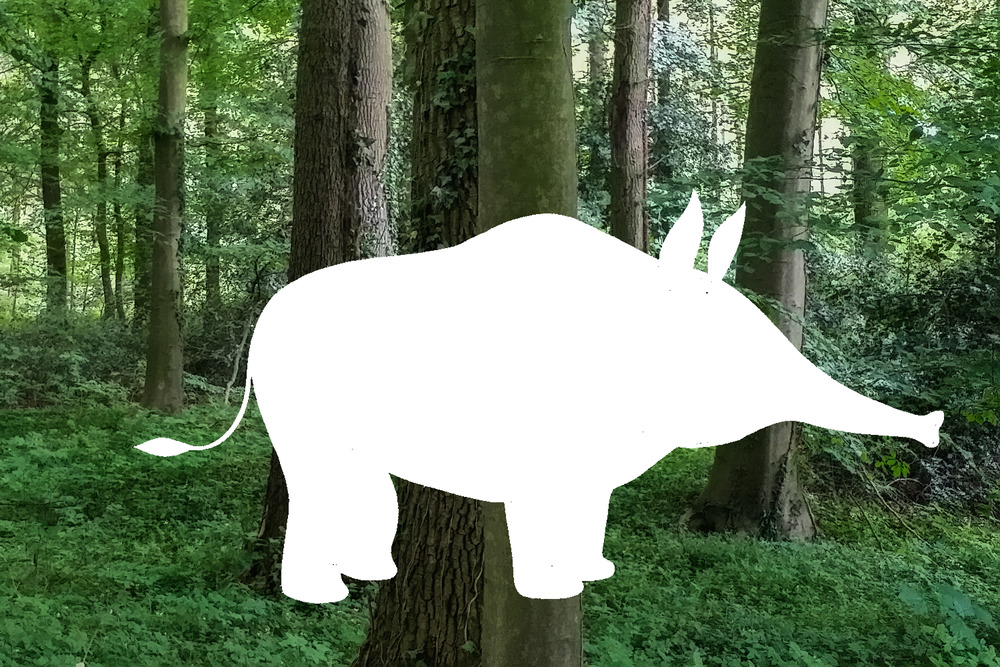
\includegraphics[width=0.45\textwidth]{bsp-1}
\subsection{Beispiel 4}
	\centering
	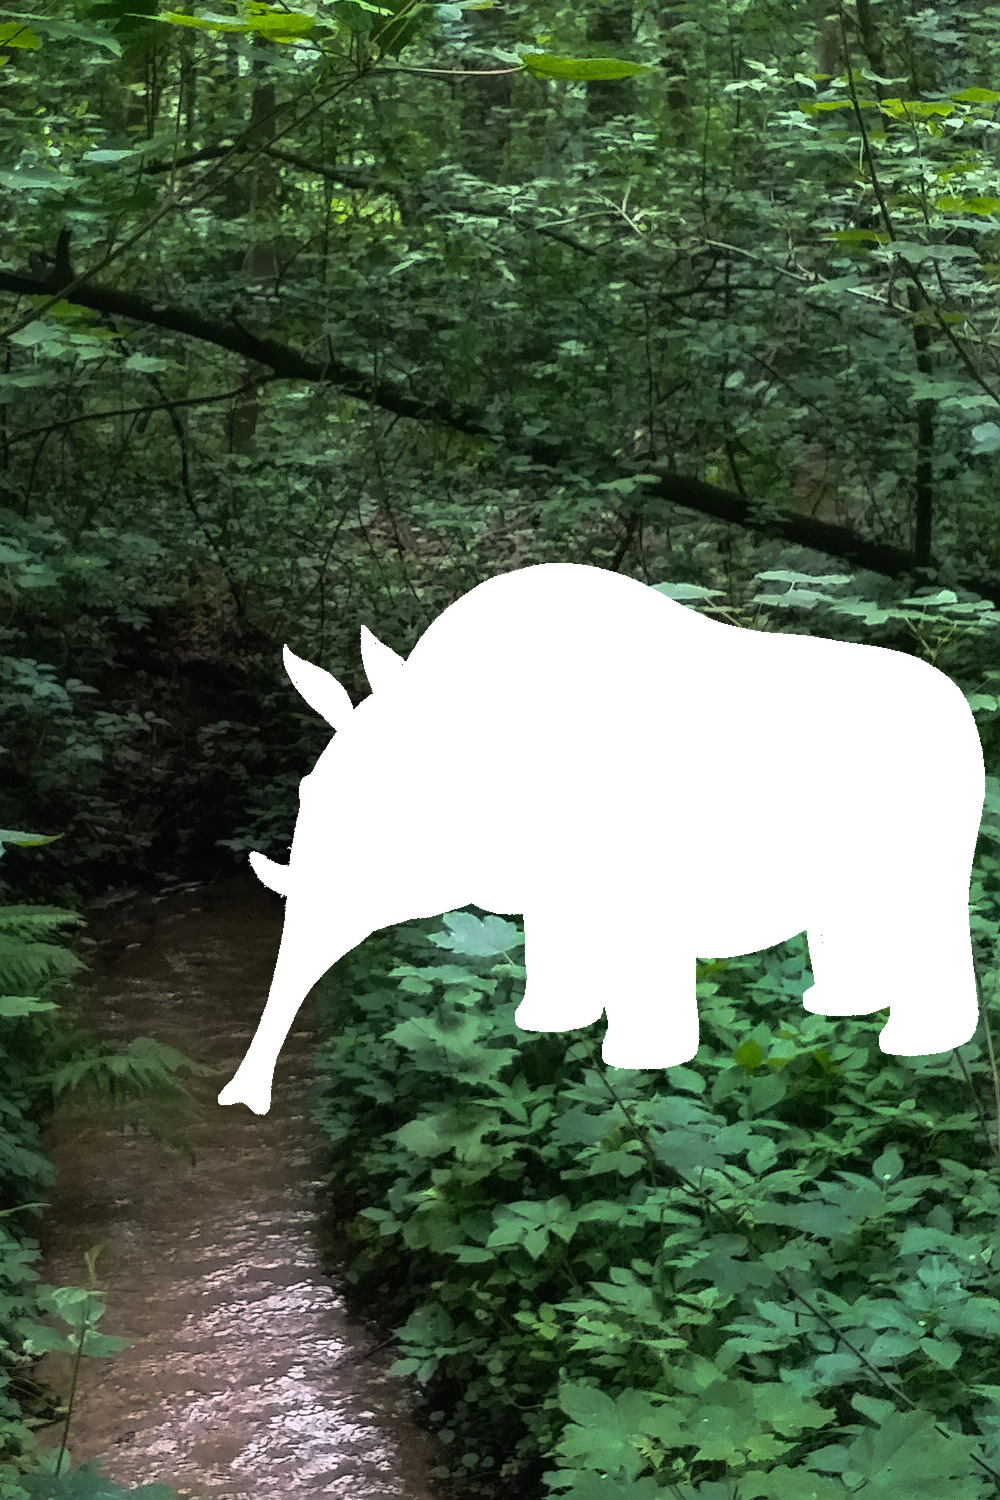
\includegraphics[width=0.45\textwidth]{bsp-2}
\subsection{Beispiel 8}
	\centering
	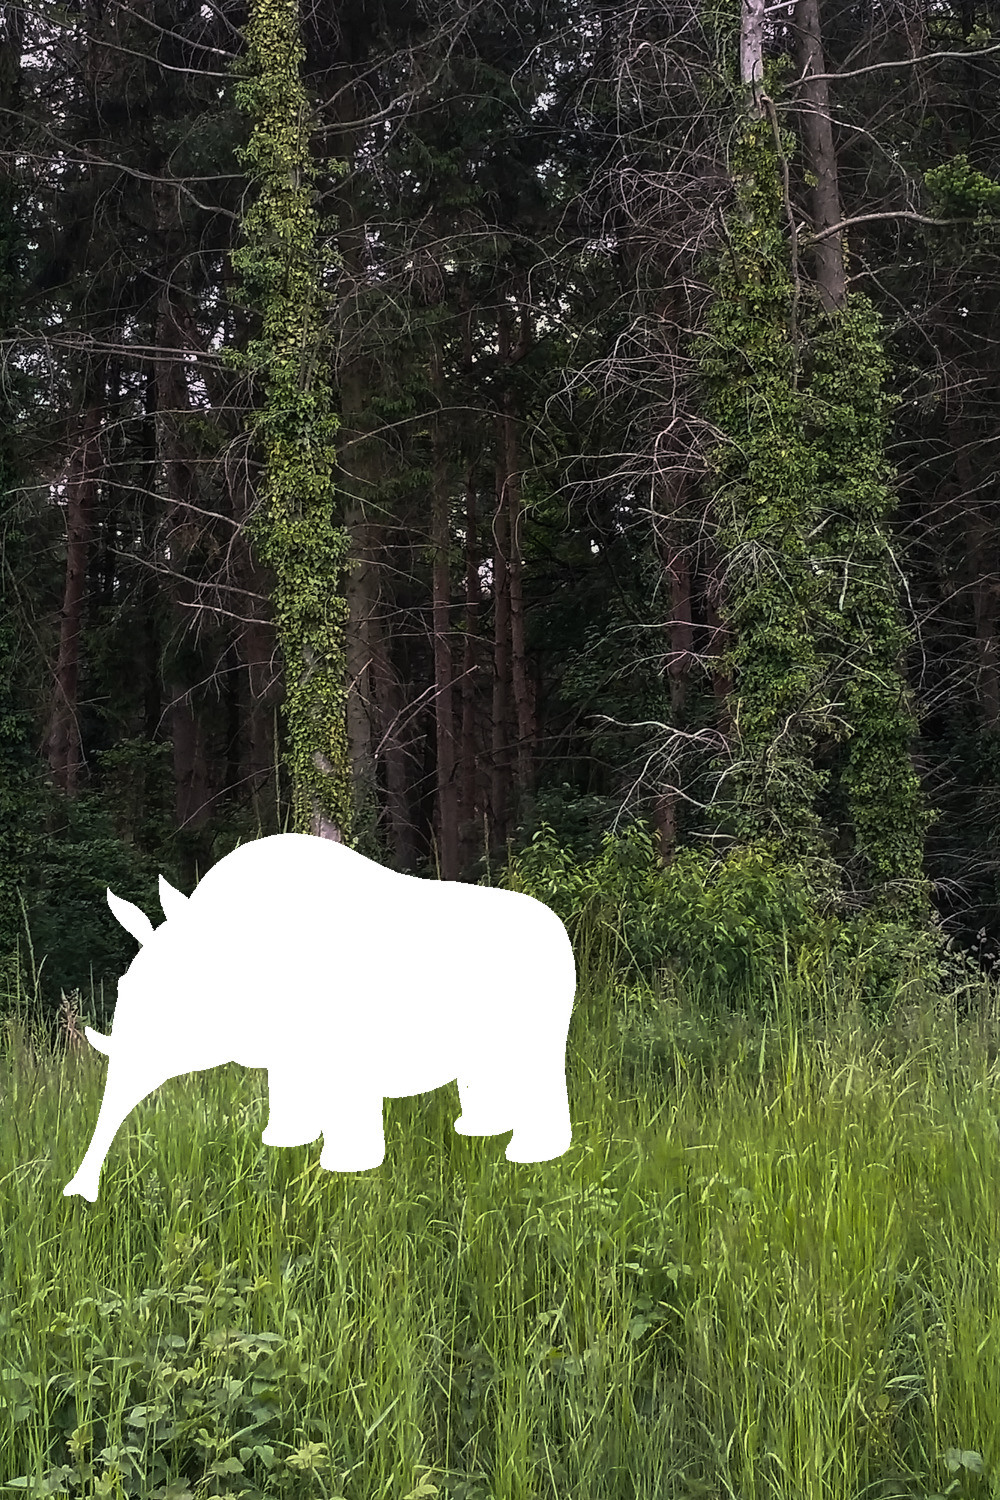
\includegraphics[width=0.45\textwidth]{bsp-3}
\subsection{Beispiel 9}
	\centering
	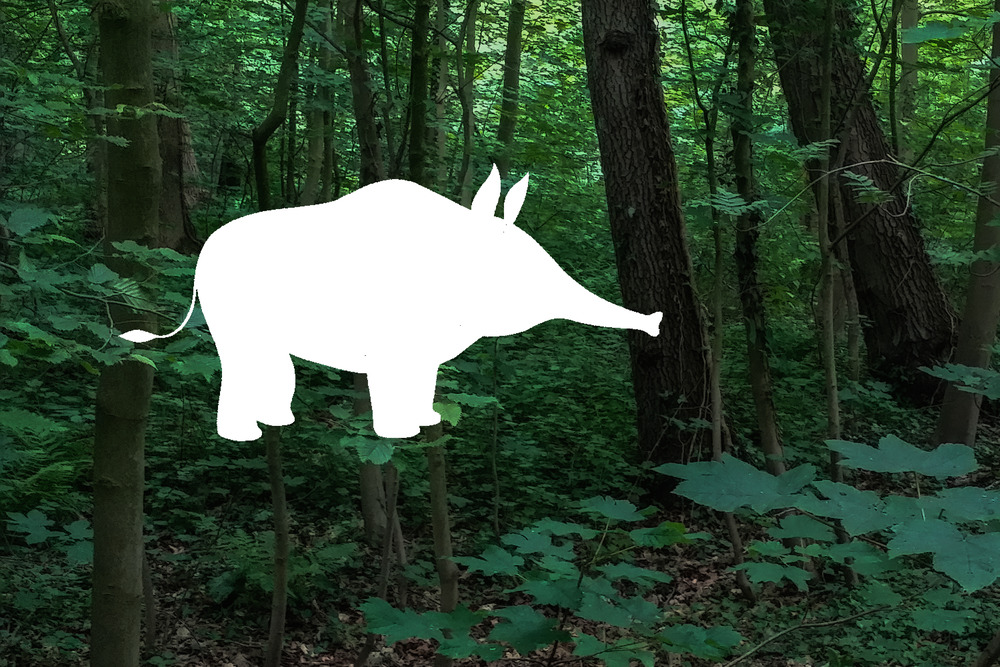
\includegraphics[width=0.45\textwidth]{bsp-4}
\end{document}